\documentclass{article}

\usepackage{graphics}
\usepackage{amsmath}
\usepackage{amsthm}
\usepackage{amsfonts}

\title{Applications: The Markov Chain Model of a 2D Map}
\author{Tzu-Chen Liang}
\date{\today}

% End of Preamble
\newtheorem{example}{Example}
\begin{document}
\maketitle
%%%%%%%%%%%%%%%%%%%%%%%%%%%%%%%%%%%%%%%%%%%%%%%%%%%%%%%%%%%%%%%%%%%%%%%%%%%%%%%%%%%%%%%%%%%%%%%%%%%%
\begin{abstract}
A section of applications and examples in the paper "Model reduction, optimal prediction, and the Mori-Zwanzig representation of Markov Chains".
\end{abstract}



%%%%%%%%%%%%%%%%%%%%%%%%%%%%%%%%%%%%%%%%%%%%%%%%%%%%%%%%%%%%%%%%%%%%%%%%%%%%%%%%%%%%%%%%%%%%%%%%%%%%
\section{Applications: The Markov Chain Model of a 2D Map}

In practice we may need to find a finite dimensional Markov chain model for a given deterministic or stochastic map $S$. This usually happens when one try to analyze some nonlinear, espcially chaotic, systems, or the map $S$ is obtained by some experimental/simulated data and do not have an analytical form. In such situations, a Markov chain model is a much easier way to evolve the system because only matrix-vector multiplications are involved. In this section we will show how to use the techniques we derived in section X to find the optimal model of such maps, espically for maps on two torus ($S: T^2 \rightarrow T^2$). Also, two examples are given.    


Let $S:T^2 \rightarrow T^2$ be the given map and $\pi$ satisfying $S(\pi)=\pi$ is a non-vanishing invariant distribution. Define function $[d_h]: T^2 \rightarrow \mathbb{R}^{1/h^2}$ to be the conditional observation of a real function on $T^2$ to finite state space $\mathbb{R}^{1/h^2}$, which can be chosen freely. However, for simplicity, the regular mesh grids on $T^2$ with grid size $h$ on each direction is used, so there are totally $1/h^2$ states numbered from $1$ to $1/h^2$. For any scalar density function on $T^2$, the function $[d_h]$ is defined as,
\begin{eqnarray}
[d_h]c(\mathbf{x}) = c
\end{eqnarray}
where $c\in \mathbb{R}^{1/h^2}$ and $c_i = \int_{a_i} c(\mathbf{x}) \text{d}a$ for $i = 1,2,...1/h^2$, and $a_i$ stands for the $i_{th}$ grid. 

The rest work is simply to match the above setting with the results we have derived. let $X = T^2$, $Y = \mathbb{R}^{1/h^2}$. It is easy to see that 
\begin{eqnarray}
\Psi_Y &=& [d_h]^T\\
\Psi_X &=& \text{diag}([d_h]\pi)^{-1}[d_h]\text{diag}(\pi)
\end{eqnarray}
and hence using (13)
\begin{eqnarray}
\bar{P} = \text{diag}([d_h]\pi)^{-1}[d_h]\text{diag}(\pi) [P] [d_h]^T
\end{eqnarray}
where $[P]$ is the Frobenious-Perron operator of $S$. For a non-singular (invertible measure-preserving) map $S$, it satisfies
\begin{eqnarray}
\label{FPoperator}
  [P]c(\mathbf{x})=c(S^{-1}(\mathbf{x}))
\end{eqnarray}
for any function $c(\mathbf{x})$. 

By noticing that $[P]^T x =S^{-1}(x) $ for any probability measure $x$, it is easier to obtain $\bar{P}^T$ first, i.e.,
\begin{eqnarray}
\bar{P}^T &=& [d_h] [P]^T \text{diag}(\pi) [d_h]^T  \text{diag}([d_h]\pi)^{-1}          
\end{eqnarray}  
and replace the $[P]^T$ above by $S^{-1}$ in computation.

Moreover, one can work out the entries of $\bar{P}$ explicitly,
\begin{eqnarray}
\label{P definition}
     \bar{P}_{ij} = \frac{\int_{S^{-1}(a_i) \cap a_j  } \pi(\mathbf{x})da}{\int_{a_i} \pi(\mathbf{x}) \text{d}a 
     } \mbox{   , for } i,j = 1,...,1/h^2
\end{eqnarray}
This will serve as our main tool for the following two examples.
Before proceeding, one should be noted that this Markov chain model is nothing more than a finite dimensional linear advection model of the underlying system with first order accuracy. The power of it is when the map $S$ and/or the observation matrix $B$ are stochastic.  

% Before that, let us first consider some computational issues of \ref{P definition}. Suppose $S$ is deterministic, the matrix $\bar{P}$ has size $n^2$ by $n^2$, and with $O(kn^2)$ nonzeros if one grid cell maps to roughly $k$ grid cells after the (inverse) map. Area integration in 2D is required for each nonzero entry, which is usually done numerically. The invariant distribution $\pi$ can be obtained by so called "bin method" or , like in our examples, knowing its phyisical meaning. 


 



%%%%%%%%%%%%%%%%%%%%%%%%%%%%%%%%%%%%%%%%%%%%%%%%%%%%%%%%%%%%%%%%%%%%%%%%%%%%%%%%%%%%%%%%%%%%%%%%%%%%
\begin{example}
Mixing Channel

The mixing process happens in a thin and long channel. Fluids with two different colors (with intensities $1$ and $0$) are injected in one end of the channel and flow through it driven by bodyforce only. The channel has some internal structure to stir the fluid passively. These structures are periodical with period $l_x$ and the cross section of the channel has dimension $l_y$ by $l_z$. The channel is assumed to be long enough so that the velocity field inside is fully developed and hence also periodical with period $l_x$. A similar mixing channel can be found in \cite{Stroock2002}.

Due to the periodical velocity field, we need only to solve it for one period, and can use this velocity field to carry the fluid with different colors iteratively to observe the mixing process at the end of each period. In fact, having the numerical velocity field, one can integrate them to get the streamlines that connect the two ends ($x=0$ and $x=l_x$) of one period length channel and define a map $S$ numerically. 

Note that the map $S$ contains no molecular diffusion information, so it does not really mix the colors. One obvious way to simulate the system is to evolve the boundary of the two colors by $S$. However, because the goal of this channel is to mix them, one can certainly image the exponentially growth of the boundary length, which increases the cost dramatically after several iterations. On the other hand, by obtaining a Markov chain model by \ref{P definition}, the reduced model can be easily evolved. Because the Markov model is always diffusive, it not only catches the evolution of the color boundary correctly at most of the iterations, but also mix the colors by the numerical diffusion.     

The mixing channel is shown in figure \ref{mixingchannel}. The simulation of the above two methods are shown in figure \ref{mixingcrosssection} for $t=1,10, 50 100, 150, 200, 250$ and $300$.


\begin{figure}
 \centerline{
  \scalebox{0.5}[0.5]{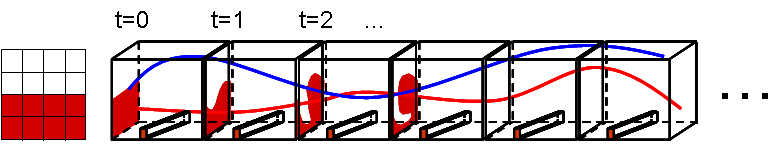
\includegraphics{mixingchannel.png}}}
  \caption{the mixing channel}
  \label{mixingchannel}
\end{figure}
 
\begin{figure}
 \centerline{
  \scalebox{0.7}[0.7]{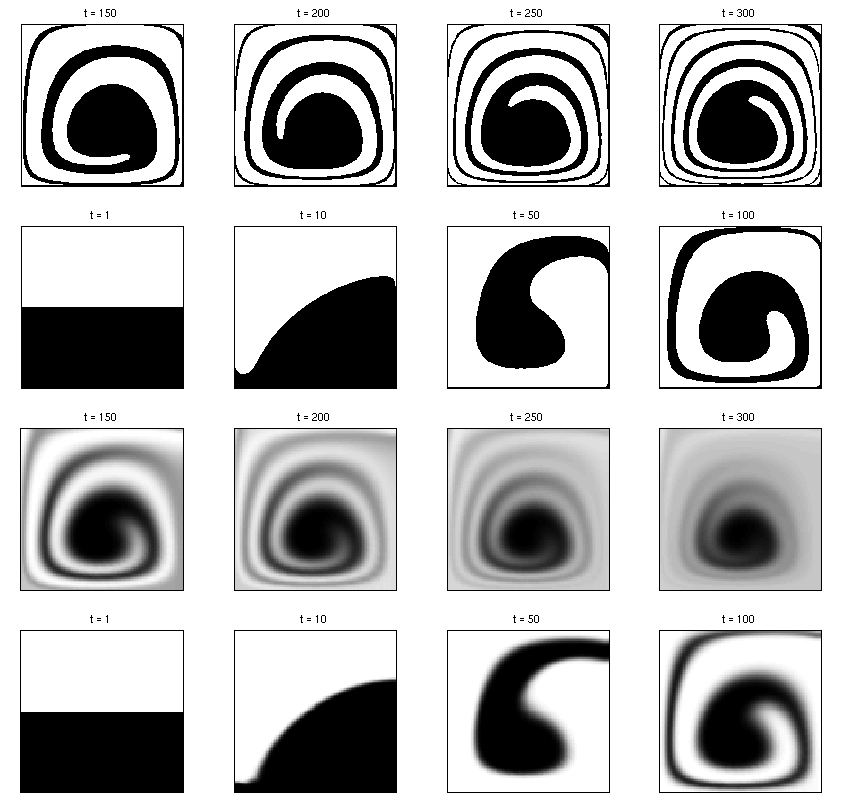
\includegraphics{mixingcrosssection.png}}}
  \caption{The cross section}
  \label{mixingcrosssection}
\end{figure}
  

\end{example}
%%%%%%%%%%%%%%%%%%%%%%%%%%%%%%%%%%%%%%%%%%%%%%%%%%%%%%%%%%%%%%%%%%%%%%%%%%%%%%%%%%%%%%%%%%%%%%%%%%%%
\begin{example}
Standard Map
\end{example}
%%%%%%%%%%%%%%%%%%%%%%%%%%%%%%%%%%%%%%%%%%%%%%%%%%%%%%%%%%%%%%%%%%%%%%%%%%%%%%%%%%%%%%%%%%%%%%%%%%%%%


%%%%%%%%%%%%%%%%%%%%%%%%%%%%%%%%%%%%%%%%%%%%%%%%%%%%%%%%%%%%%%%%%%%%%%%%%%%%%%%%%%%%%%%%%%%%%%%%%%%%
\section{Random Walk on a Hypercube and the Ehrenfests' Urn}

It is easy to check that the reduced system is exact if the following condition holds,

\begin{eqnarray}
 (\Psi_X^T\Psi_Y^T-I)(P^T)^t x(0) =0 \mbox{  , for }t=0,1,...
\end{eqnarray}
i.e., $x(t)$ evolves in the null space of $\Psi_X^T\Psi_Y^T-I$. Suppose $P$ is full rank (no redundant states in the original Markov chain), the selection of observation matrix $B$ is clearly related to the initial state $x(0)$. The appropriate choice of $B$ with respect to some special $x(0)$ is not easy but can reduce a large Markov chain to a much smaller one and still keeps the desired proterties. This kind of technique is (perhaps) widely used in the study of Markov chain problems. Here are two examples. 


Consider the Random walk on an $n$-dimensional hypercube: a particle starts at $\mathbf{0}$ and moves to one of its nearest neighbors (or stay fixed) with equal probability at each step. This can be simply modeled as a Markov chain with $2^n$ state\cite{Diaconis1990}. However, one can also set the states to be the 1-norm distance to the orgin. For example, on a 3-d cube, the corners with coordinates $(0,0,0)$, $(0,1,0)$ and $(1,0,1)$ are at states $0$,$1$ and $2$, respectively. The observation matrix $B$ is thus,
\begin{eqnarray}
B_{ij} = \left\{ \begin{array}{cc}
                 1,&\mbox{ if } i_{th} \mbox{ corner has 1-norm distance } j \mbox{ to the origin}\\
                 0,&\mbox{ otherwise}
                 \end{array} \right.
\end{eqnarray}



This reduces the number of states from $2^n$ to $n$. The new problem is called Ehrenfests' Urn problem and has also been widely studied. 

When one simulates both systems starting at state $\mathbf{0}$ and $0$, the following holds,
\begin{eqnarray}
y(t) = B^T x(t) \mbox{  , for } t={0,1,...} 
\end{eqnarray} 
i.e., for this particular initial condition, the model reduction is exact. This fact has been used in the study of the cut-off phenomenon in finite Markov chain. 

%%%%%%%%%%%%%%%%%%%%%%%%%%%%%%%%%%%%%%%%%%%%%%%%%%%%%%%%
The same reduction is applied to the analysis of riffle shuffling. Riffle shuffle is the most common method of mixing cards. A deck of $n$ cards (often $n=52$) is cut into two parts and the parts are riffled together. The basic model of this procedure was introduced by Gilbert and Shannon(1955)\cite{Gilbert1955}. A good review of related studies and its interesting phenomenon called cutoff can be found in \cite{Diaconis2001}. In this model, the deck is cut into two piles according to the binomial distribution so the chance that pile one has $j$ cards is ${n \choose j}/2^n$. Then, sequentially drop cards from the bottoms of the two piles according to the following rule: if at some stage pile one has $A$ cards and pile two has $B$ cards, drop the next card from pile one with probability $A/(A+B)$. This is continued until the two piles are exhausted and then the piles are pushed together. This defines a Markov chain with $n!$ states (permutations). However, Bayer and Diaconis\cite{Diaconis1992} showed that it is enough to study only the number of rising sequences of the permutations, i.e, using the followeing deterministic observation $B$,

    
\begin{eqnarray}
B_{ij} = \left\{ \begin{array}{cc}
                 1,&\mbox{ if } i_{th} \mbox{ permutation has } j \mbox{ rising sequence}\\
                 0,&\mbox{ otherwise}
                 \end{array} \right.
\end{eqnarray}

The reduced system has $n$ states only, and again, when the initial permutation has only one rising sequence, the two Markov chains behave the same. 


%%%%%%%%%%%%%%%%%%%%%%%%%%%%%%%%%%%%%%%%%%%%%%%%%%%%%%%

% References
\bibliographystyle{plain}
\bibliography{mixingchannelexamplebib} 

\cite{Stroock2002}
\cite{Diaconis1990}
\cite{Diaconis2001}
\cite{Diaconis1986}
\cite{Diaconis1992}

\cite{Gilbert1955}











\end{document}
